% ============================================================
%  Analog Color Measurement — Combined Writeup
%  Paste into Overleaf (pdfLaTeX, no extra packages needed
%  beyond the standard ones listed below).
% ============================================================
\documentclass[11pt, letterpaper]{article}

% --- Packages -----------------------------------------------
\usepackage[margin=1in]{geometry}
\usepackage{amsmath, amssymb}
\usepackage{graphicx}
\usepackage{booktabs}
\usepackage{hyperref}
\usepackage{caption}
\usepackage{subcaption}
\usepackage{float}
\usepackage{listings}
\usepackage{xcolor}
\usepackage{tikz}
\usetikzlibrary{shapes.geometric, arrows.meta, positioning, calc}

% --- Metadata -----------------------------------------------
\title{\textbf{Analog Color Measurement}\\[4pt]
       \large Capturing and Modeling Hardware Nonlinearities\\
       as Deployable Audio Plugins}
\author{John Micensky}
\date{\today}

% ============================================================
\begin{document}
\maketitle
\tableofcontents
\newpage

% ------------------------------------------------------------
\section{Introduction}
\label{sec:intro}
% TODO: Motivate the problem. Why does analog "color" matter?
% What gap does this tool fill vs. existing impulse-response
% capture workflows (which only model linear behavior)?

% ------------------------------------------------------------
\section{Background and Related Work}
\label{sec:background}
% TODO: Brief survey of:
%   - Hammerstein / Wiener / L-N-L cascade models in audio literature
%   - Existing hardware emulation approaches (convolution, circuit simulation)
%   - Limitations of linear IR capture for saturating devices

% ------------------------------------------------------------
\section{System Overview}
\label{sec:system}

The measurement system is implemented as a JUCE standalone desktop application.
The tool captures analog audio nonlinearities (\emph{color}) from hardware
devices and models them as deployable audio plugins.
Figure~\ref{fig:system_flow} gives a high-level view of the signal flow from
hardware device under test through to the exported plugin model.

% --- Block diagram placeholder ---
\begin{figure}[H]
    \centering
    % TODO: replace with a real TikZ or inkscape figure
    \fbox{\parbox{0.8\textwidth}{\centering\vspace{1.5cm}
          [System block diagram: Device Under Test $\to$ ADC $\to$
           Capture Pipeline $\to$ Analysis Engine $\to$ LNL Model $\to$ Plugin]\vspace{1.5cm}}}
    \caption{End-to-end signal flow of the measurement and modeling pipeline.}
    \label{fig:system_flow}
\end{figure}

\subsection{Application Architecture}
% TODO: Describe the major software components:
%   MainComponent (UI), AudioEngine (real-time I/O),
%   StimulusPlan (test sequence), SessionWriter (disk I/O),
%   AnalysisEngine (offline), LNLModel (data structure), Plugin target.

\subsection{Session Outputs}
Each measurement session produces four artifacts per stimulus step:
\begin{itemize}
    \item \texttt{*\_ref.wav} — the direct reference signal recorded simultaneously with playback
    \item \texttt{*\_rec.wav} — the return signal captured from the hardware device
    \item \texttt{session.json} — metadata (device name, sample rate, gain labels, timestamps)
    \item \texttt{markers.json} — per-step index mapping filenames to gain settings and stimuli
\end{itemize}

% ------------------------------------------------------------
\section{Stimulus Design}
\label{sec:stimulus}

Measurements are organized into a \emph{stimulus plan}: an ordered sequence of
$(g, s)$ pairs where $g$ is a hardware gain setting and $s$ is one of the
available test stimuli.  Three quality tiers are defined:

\begin{table}[H]
    \centering
    \begin{tabular}{lll}
        \toprule
        \textbf{Quality} & \textbf{Stimuli} & \textbf{Purpose} \\
        \midrule
        Quick    & Sine sweep, 1\,kHz sine                                      & Fast sanity check \\
        Standard & Sine sweep, 1\,kHz sine, 100\,Hz sine, drums excerpt         & Balanced coverage \\
        HiFi     & Sine sweep, pink noise, 1\,kHz, 100\,Hz, drums excerpt       & Full characterization \\
        \bottomrule
    \end{tabular}
    \caption{Stimulus quality tiers and their constituent signals.}
    \label{tab:quality}
\end{table}

% TODO: Add rationale for each stimulus choice (e.g., why 100 Hz specifically,
% why a real drums excerpt rather than a second sine).

% ------------------------------------------------------------
\section{Latency Alignment}
\label{sec:latency}

Before any analysis, the recorded signal $r[n]$ must be time-aligned with the
reference signal $x[n]$ to compensate for round-trip hardware latency.
The integer-sample delay $\hat{\tau}$ is estimated via normalized
cross-correlation:

\begin{equation}
    \hat{\tau} \;=\; \arg\max_{\tau} \;
    \frac{\displaystyle\sum_{n} x[n]\, r[n - \tau]}
         {\sqrt{\displaystyle\sum_{n} x[n]^{2}\;
                \displaystyle\sum_{n} r[n]^{2}}}
    \label{eq:xcorr}
\end{equation}

The alignment is computed efficiently in the frequency domain using the FFT:

\begin{equation}
    C[k] \;=\; X[k] \cdot R^{*}[k],
    \qquad
    c[n] \;=\; \mathcal{F}^{-1}\!\left\{C[k]\right\},
    \qquad
    \hat{\tau} \;=\; \arg\max_{n}\; c[n]
    \label{eq:xcorr_fft}
\end{equation}

% TODO: Report measured latency values on your test interface.
% TODO: Discuss sub-sample interpolation if implemented.

% ------------------------------------------------------------
\section{Gray-Box L--N--L Model}
\label{sec:lnl}

\subsection{Model Motivation}
\label{sec:lnl_motivation}

A purely \emph{black-box} model (e.g., a deep neural network trained end-to-end)
can achieve high accuracy but offers no interpretability and is expensive to
deploy in real-time audio contexts.  A purely \emph{white-box} model (e.g., a
full circuit simulation) is physically accurate but requires proprietary
schematic knowledge and is computationally prohibitive at audio rates.

This project adopts a \emph{gray-box} approach: the model topology is fixed by
prior knowledge of analog signal chains (a cascade of linear filtering and a
static nonlinearity), while the parameters of each block are estimated
empirically from the captured data.

\subsection{Model Structure}
\label{sec:lnl_structure}

The device under test is modeled as a \emph{Linear--Nonlinear--Linear} (L--N--L)
cascade, illustrated in Figure~\ref{fig:lnl_diagram}.

\begin{figure}[H]
\centering
\begin{tikzpicture}[
    block/.style = {rectangle, draw, minimum width=2.2cm, minimum height=1cm,
                    text centered, font=\small},
    line/.style  = {draw, -{Stealth[length=2mm]}}
]
    \node[block]                       (l1) {$L_1[z]$\\{\tiny Input Filter}};
    \node[block, right=1.4cm of l1]    (n)  {$\mathcal{N}(\cdot)$\\{\tiny Waveshaper}};
    \node[block, right=1.4cm of n]     (l2) {$L_2[z]$\\{\tiny Output Filter}};

    \coordinate (in)  at ([xshift=-1.4cm]l1.west);
    \coordinate (out) at ([xshift=+1.4cm]l2.east);

    \line (in)    -- node[above]{\small$x[n]$} (l1.west);
    \line (l1.east) -- node[above]{\small$v[n]$} (n.west);
    \line (n.east)  -- node[above]{\small$w[n]$} (l2.west);
    \line (l2.east) -- node[above]{\small$\hat{y}[n]$} (out);
\end{tikzpicture}
\caption{L--N--L gray-box model. The input signal $x[n]$ passes through a
linear FIR filter $L_1$, a static memoryless nonlinearity $\mathcal{N}$,
and a second linear FIR filter $L_2$ to produce the model output
$\hat{y}[n]$.}
\label{fig:lnl_diagram}
\end{figure}

The model output is:

\begin{equation}
    \hat{y}[n] \;=\; \bigl(h_2 * \mathcal{N}(h_1 * x)\bigr)[n]
    \label{eq:lnl}
\end{equation}

where $h_1$ and $h_2$ are the FIR impulse responses of $L_1$ and $L_2$
respectively, $*$ denotes linear convolution, and $\mathcal{N}$ is a
point-wise static function.

\subsection{Block Identification}
\label{sec:lnl_id}

Each block is identified independently from dedicated measurements.

\paragraph{$L_1$: Input Filter.}
The linear frequency response of the device is measured using a sine sweep
stimulus.  The transfer function magnitude is estimated bin-wise as:

\begin{equation}
    \bigl|\hat{H}(f_k)\bigr| \;=\;
    \frac{\bigl|\mathcal{F}\{r\}[k]\bigr|}{\bigl|\mathcal{F}\{x\}[k]\bigr|}
    \label{eq:fr_estimate}
\end{equation}

where $x$ and $r$ are the (aligned) reference and recorded signals.
The magnitude spectrum is 1/3-octave smoothed and used to design a
$512$-tap linear-phase FIR filter $h_1$ via an inverse-FFT window method.
Full implementation details are given in Section~\ref{sec:analysis_fr}.

\paragraph{$\mathcal{N}$: Static Nonlinearity (Waveshaper).}
With $L_1$ applied, the pre-filtered signal $v[n] = (h_1 * x)[n]$ is
compared to the recorded output at each sample amplitude.  The mapping
$v[n] \mapsto r[n]$ is accumulated into a 1024-entry lookup table
(waveshaper) uniformly spanning the input range $[-1,\,+1]$:

\begin{equation}
    \mathcal{N}(a) \;\approx\; \text{LUT}\!\left[
        \left\lfloor \frac{(a + 1)}{2} \cdot 1023 \right\rceil
    \right]
    \label{eq:waveshaper}
\end{equation}

Measurements at multiple gain levels and stimulus frequencies (100\,Hz and
1\,kHz sine tones) are pooled to improve coverage of the input amplitude range.
Implementation details are given in Section~\ref{sec:analysis_ws}.

\paragraph{$L_2$: Output Filter.}
In the current implementation $L_2$ is the identity ($h_2 = \delta$).
A non-trivial output filter may be fitted in future work to capture
output-side coloration that is not attributable to the input chain or
the nonlinearity.

\subsection{Total Harmonic Distortion}
\label{sec:thd}

As a diagnostic, Total Harmonic Distortion (THD) is computed for each
sine-tone capture:

\begin{equation}
    \text{THD} \;=\;
    \frac{\sqrt{\displaystyle\sum_{k=2}^{K} A_k^2}}{A_1} \times 100\%
    \label{eq:thd}
\end{equation}

where $A_1$ is the fundamental amplitude and $A_k$ is the amplitude of the
$k$-th harmonic, all estimated from the magnitude spectrum of the recorded signal.
THD is reported per gain label to characterize the onset and degree of saturation.

\subsection{Analysis Pipeline Implementation}
\label{sec:analysis_impl}

The full LNL model is fitted offline by
\texttt{AnalysisEngine::analyseProjectFolder}.  The pipeline has two
branches, described below.

\subsubsection{Frequency Response and FIR Design ($L_1$)}
\label{sec:analysis_fr}

\begin{enumerate}
  \item \textbf{File scan.}  All \texttt{*\_SineSweep\_ref.wav} /
        \texttt{*\_SineSweep\_rec.wav} pairs in the project folder are
        located.

  \item \textbf{Transfer-function estimate.}  For each pair a 1D FFT
        of size $2^{\lceil\log_2 N\rceil}$ is computed for both the
        reference and the recording.  The pointwise magnitude ratio
        $|H[k]| = |\hat{y}_{\text{rec}}[k]| / |\hat{y}_{\text{ref}}[k]|$
        is linearly resampled onto a fixed 2049-bin design grid
        ($N_{\text{design}} = 4096$).

  \item \textbf{Averaging.}  Results from all sweep captures are
        averaged bin-by-bin to reduce noise.

  \item \textbf{Smoothing.}  A 1/3-octave running-mean smoother is
        applied to retain only the perceptually relevant spectral shape.
        The DC bin is extrapolated from the first two measured bins to
        avoid artificial discontinuities at low frequencies caused by
        the absence of DC energy in the sweep signal.

  \item \textbf{Quality gate.}  If the 1\,kHz magnitude bin is below
        $-40$\,dB (linear amplitude $< 0.01$), the sweep data is judged
        invalid and the model falls back to an identity FIR.

  \item \textbf{Normalisation.}  The spectrum is normalised to unity
        gain at 1\,kHz so the FIR models the device's spectral
        \emph{shape} relative to 1\,kHz, not the absolute recording chain gain.

  \item \textbf{FIR design.}  A 512-tap linear-phase FIR is synthesised
        using the zero-phase IFFT method: the smoothed half-spectrum is
        reflected into a symmetric full spectrum, a 4096-point inverse
        FFT yields the zero-phase impulse response, and the centre 512
        samples are extracted and multiplied by a Hann window.

  \item \textbf{Stored display data.}  Every 4th bin is saved as
        \texttt{frFrequencies} / \texttt{frMagnitudeDb} in the model for
        display purposes and for FIR reconstruction at alternate sample
        rates (see Section~\ref{sec:artifact_loading}).
\end{enumerate}

\subsubsection{Waveshaper and THD ($\mathcal{N}$)}
\label{sec:analysis_ws}

\begin{enumerate}
  \item \textbf{File scan.}  All \texttt{*\_Sine1kHz\_*} and
        \texttt{*\_Sine100Hz\_*} capture pairs, across all gain-level
        sub-folders, are located.

  \item \textbf{THD measurement.}  For each capture, a 65536-point
        FFT (order~16) is computed on a Hann-windowed excerpt drawn from
        the middle of the recording to avoid onset and release transients.
        The fundamental bin is located within $\pm 10$ bins of the nominal
        frequency; power in harmonics~2 through~9 is summed to compute THD
        per (\ref{eq:thd}).  The gain label (parent folder name,
        e.g.\ ``75\%'') and fundamental amplitude in dBFS are stored
        alongside each THD result.

  \item \textbf{Waveshaper scatter.}  For each sample~$n$ in the same
        analysis window, the reference sample $x[n]$ is mapped to one of
        1024 uniformly-spaced bins over $[-1,\,+1]$ and the corresponding
        recorded sample $y[n]$ is accumulated.  After all captures, the
        per-bin average becomes the waveshaper table entry.

  \item \textbf{Gap filling.}  Bins with zero hits (amplitudes never
        reached by the test signal) are filled by linear interpolation
        between populated neighbours.  Extreme bins outside the populated
        region are extrapolated linearly using the slope measured at the
        nearest populated edge, which correctly handles phase-inverting
        devices that would otherwise produce an artificial gain drop at
        high drive.

  \item \textbf{Small-signal normalisation.}  The slope of the
        waveshaper around $x = 0$ (averaged over a $\pm 8$-sample window
        about the table centre) is divided out so the table's small-signal
        gain equals~1.  This isolates the nonlinear character from the
        recording chain's absolute gain, consistent with the 1\,kHz
        normalisation applied to the FIR.
\end{enumerate}

% ------------------------------------------------------------
\section{Measurement Procedure}
\label{sec:procedure}
% TODO: Step-by-step instructions a reader would follow to
% characterize a new device. Reference the UI workflow.

% ------------------------------------------------------------
\section{Plugin Implementation}
\label{sec:plugin}

The Hardware Color plugin (\texttt{HardwareColorProcessor}) is a stereo
VST3/AU AudioProcessor that loads a fitted LNL artifact at runtime and
applies it to the incoming audio stream.

\subsection{Signal Chain}
\label{sec:plugin_chain}

The per-channel processing path, executed each block in
\texttt{processBlock}, is illustrated in Figure~\ref{fig:plugin_chain}.

\begin{figure}[H]
\centering
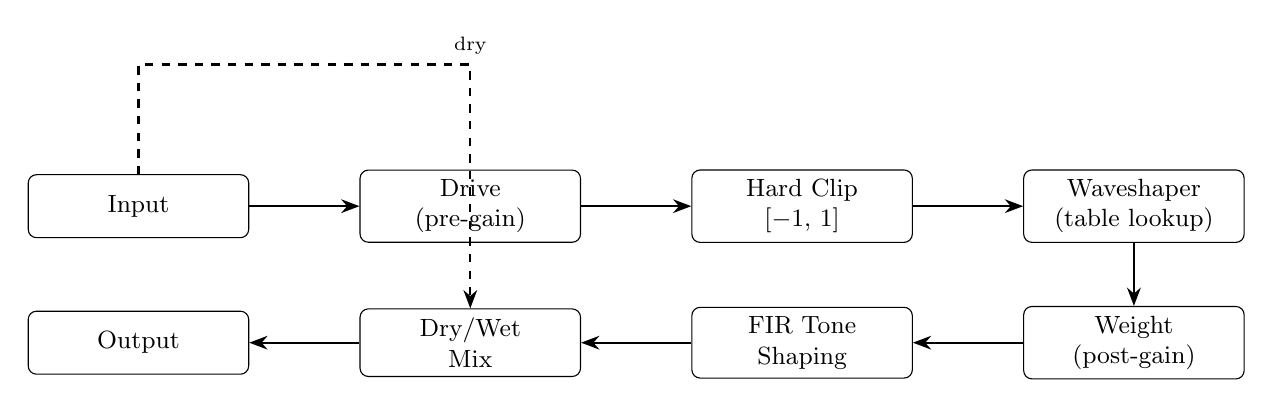
\begin{tikzpicture}[
    node distance = 8mm and 14mm,
    box/.style    = {rectangle, draw, rounded corners=3pt,
                     minimum width=28mm, minimum height=8mm,
                     font=\small, align=center},
    arr/.style    = {-Stealth, thick}
]
  \node[box] (in)    {Input};
  \node[box, right=of in]  (drive)  {Drive\\(pre-gain)};
  \node[box, right=of drive] (clip)  {Hard Clip\\{$[-1,\,1]$}};
  \node[box, right=of clip]  (ws)    {Waveshaper\\(table lookup)};
  \node[box, below=of ws]    (wt)    {Weight\\(post-gain)};
  \node[box, left=of wt]     (fir)   {FIR Tone\\Shaping};
  \node[box, left=of fir]    (mix)   {Dry/Wet\\Mix};
  \node[box, left=of mix]    (out)   {Output};

  \draw[arr] (in)    -- (drive);
  \draw[arr] (drive) -- (clip);
  \draw[arr] (clip)  -- (ws);
  \draw[arr] (ws)    -- (wt);
  \draw[arr] (wt)    -- (fir);
  \draw[arr] (fir)   -- (mix);
  \draw[arr] (mix)   -- (out);

  % dry tap
  \coordinate (tap) at ($(in)!0.5!(drive) + (0,18mm)$);
  \draw[arr, dashed] (in.north) |- (tap) -| (mix.north)
        node[midway, above, font=\scriptsize] {dry};
\end{tikzpicture}
\caption{Per-channel signal chain in the Hardware Color plugin.  The dry
tap precedes Drive so that Mix provides a true parallel blend independent
of the other two controls.}
\label{fig:plugin_chain}
\end{figure}

\noindent
The numbered processing steps per sample are:
\begin{enumerate}
  \item Multiply sample by Drive.
  \item Hard-clip to $[-1,\,1]$.
  \item Look up the result in the 1024-entry waveshaper table using
        linear interpolation between adjacent entries.
  \item Multiply by Weight.
  \item Convolve with the 512-tap FIR (applied \emph{post-saturation}
        so it shapes the distorted output's harmonic content rather than
        pre-filtering the clean input).
  \item Blend with the stored dry sample at the Mix ratio.
\end{enumerate}

FIR convolution uses a direct-form delay-line implementation.  A
per-channel history buffer of length $\text{taps} - 1$ is maintained
across blocks and reset on model load or channel-count change.

\subsection{Controls}
\label{sec:plugin_controls}

The plugin exposes three automatable parameters via
\texttt{AudioProcessorValueTreeState}.

\subsubsection{Drive}

\begin{description}
  \item[Range] $0.0 \;\text{--}\; 10.0$ \quad Default: $1.0$ \quad Step: $0.01$
\end{description}

Drive is a pre-gain scalar applied to every sample before the waveshaper:
\[
  x_{\text{in}} = s[n] \times d_{\text{drive}}
\]
The result is hard-clipped to $[-1,\,1]$ before the waveshaper lookup.
At the default value of $1.0$ the signal enters at the amplitude it was
captured at, reproducing the measured behaviour exactly.  Values
above~$1.0$ push more of the waveform into the saturating region of the
waveshaper curve; values below~$1.0$ keep the signal in the more linear
small-signal regime.

\subsubsection{Weight}

\begin{description}
  \item[Range] $0.0 \;\text{--}\; 2.0$ \quad Default: $1.0$ \quad Step: $0.01$
\end{description}

Weight is a post-nonlinearity output scalar:
\[
  s_{\text{ws}}[n] = \textsc{Waveshaper}(x_{\text{in}}) \times w_{\text{weight}}
\]
It controls the level of the coloured signal \emph{after} the waveshaper,
before FIR tone shaping and dry/wet mixing.  At $1.0$ the waveshaper's
small-signal gain — which was normalised to unity during analysis — is
preserved.  Raising Weight brightens the wet signal's level without
altering the nonlinear character; lowering it fades the coloured path
while the dry path (tapped before Drive) remains unaffected.

\subsubsection{Mix}

\begin{description}
  \item[Range] $0.0 \;\text{--}\; 1.0$ \quad Default: $1.0$
\end{description}

Mix is a linear dry/wet blend applied after all tone shaping:
\[
  s_{\text{out}}[n] = s_{\text{dry}}[n]\,(1 - m) \;+\; s_{\text{wet}}[n]\, m
\]
where $s_{\text{dry}}$ is the signal captured before Drive and
$s_{\text{wet}}$ is the FIR-shaped, weighted output.  At $1.0$ only the
processed signal is heard; at $0.0$ the plugin is fully transparent.
Because the dry tap precedes Drive, Mix acts as a true parallel blend
regardless of Drive or Weight settings.

\subsection{Artifact Loading and Sample-Rate Adaptation}
\label{sec:artifact_loading}

The plugin loads an artifact file at any time from the message thread via
\texttt{loadArtifact}.  The artifact bundles:
\begin{itemize}
  \item \textbf{FIR coefficients} (512 taps) derived from the device's
        measured frequency response.
  \item \textbf{Waveshaper table} (1024 entries) mapping input amplitude
        to output amplitude over $[-1,\,+1]$.
  \item \textbf{Downsampled frequency-response data} (magnitude vs.\
        frequency in Hz / dB) for FIR reconstruction and display.
  \item \textbf{THD measurements} per tone and gain level (display only).
\end{itemize}

If the DAW's current sample rate differs from the model's capture rate by
more than 1\,Hz, the FIR is rebuilt immediately via
\texttt{AnalysisEngine::rebuildFirAtSampleRate}.  This routine
interpolates the stored frequency-response data onto a new design grid at
the target rate and re-runs the linear-phase FIR design, ensuring the
tone-shaping response is accurate at 44.1\,kHz, 48\,kHz, 88.2\,kHz, and
96\,kHz sessions.  The same check runs in \texttt{prepareToPlay} so that
a session opened at a different rate than the artifact's capture rate is
corrected automatically.

% ------------------------------------------------------------
\section{Results}
\label{sec:results}
% TODO: Apply to a specific hardware device.
% Include FR plot, THD vs. gain table, waveshaper curve,
% and A/B perceptual evaluation.

\subsection{Frequency Response}
% TODO: Figure — measured vs. modeled FR.

\subsection{Nonlinearity Characterization}
% TODO: Figure — waveshaper curve + THD table.

\subsection{Perceptual Evaluation}
% TODO: Informal listening test methodology and findings.

% ------------------------------------------------------------
\section{Discussion}
\label{sec:discussion}
% TODO: Model limitations (memory effects, dynamic nonlinearities,
% compressor behavior not yet captured). Future work.

% ------------------------------------------------------------
\section{Conclusion}
\label{sec:conclusion}
% TODO: Summarize contributions and outcomes.

% ------------------------------------------------------------
\bibliographystyle{plain}
\bibliography{refs}
% TODO: populate refs.bib with relevant citations.

\end{document}
